\section{Browser-Technologien}

\subsection{Vordefinierte Browser-Objekte}

\begin{definition}{Browser-Objekte}\\
    Im Browser stehen spezielle globale Objekte zur Verfügung:
    \begin{itemize}
        \item \texttt{window}: Browserfenster und globaler Scope
            \begin{itemize}
                \item \texttt{window.innerHeight}: Viewport Höhe
                \item \texttt{window.pageYOffset}: Scroll Position
                \item \texttt{window.location}: URL Manipulation
            \end{itemize}
        \item \texttt{document}: Das aktuelle HTML-Dokument
        \item \texttt{navigator}: Browser-Informationen
        \item \texttt{history}: Browser-Verlauf
        \item \texttt{location}: URL-Informationen
    \end{itemize}
\end{definition}

\begin{KR}{document-Objekt} repräsentiert das aktuelle HTML-Dokument:
\begin{lstlisting}[language=JavaScript, style=basesmol]
// Element finden
document.getElementById("id")  
document.querySelector("selector") 
document.querySelectorAll("selector")
// DOM manipulieren
document.createElement("tag")       // Element erstellen  
document.createTextNode("text")     // Textknoten erstellen
document.createAttribute("attr")    // Attribut erstellen
// Event Handler
document.addEventListener("event", handler)
\end{lstlisting}
\end{KR}

\begin{KR}{window-Objekt} als globaler Namespace:
\begin{lstlisting}[language=JavaScript, style=basesmol]
// Globale Methoden
window.alert("message")
window.setTimeout(callback, delay)
window.requestAnimationFrame(callback)
// Eigenschaften
window.innerHeight  // Viewport Hoehe
window.pageYOffset  // Scroll Position
window.location    // URL Infos
\end{lstlisting}
\end{KR}

\begin{KR}{navigator-Objekt} für Browser-Informationen:
\begin{lstlisting}[language=JavaScript, style=basesmol]
navigator.userAgent  // Browser User-Agent
navigator.language   // Browser Sprache
navigator.onLine     // Online-Status
\end{lstlisting}
\end{KR}

\begin{KR}{history-Objekt}für Browser-Verlauf:
\begin{lstlisting}[language=JavaScript, style=basesmol]
history.length  // Anzahl Eintraege
history.back()  // Zurueck zur letzten Seite
history.forward()  // Vorwaerts zur naechsten Seite
\end{lstlisting}
\end{KR}

\begin{KR}{location-Objekt} für URL-Informationen:
\begin{lstlisting}[language=JavaScript, style=basesmol]
location.href  // URL der Seite
location.hostname  // Hostname
location.pathname  // Pfad
location.search  // Query-Parameter
location.hash  // Anker
\end{lstlisting}
\end{KR} 

\subsection{Document Object Model (DOM)}

structure:
\begin{itemize}
    \item element auffinden
    \item textknoten erzeugen
    \item elementknoten erzeugen
    \item attribute setzen
    \item style anpassen
\end{itemize}

\begin{concept}{DOM Struktur}
    Das DOM ist eine Baumstruktur des HTML-Dokuments:
    \begin{itemize}
        \item Jeder HTML-Tag wird zu einem Element-Knoten
        \item Text innerhalb von Tags wird zu Text-Knoten
        \item Attribute werden zu Attribut-Knoten
        \item NodeType Konstanten:
            \begin{itemize}
                \item 1: Element Node (ELEMENT\_NODE)
                \item 3: Text Node (TEXT\_NODE)
                \item 8: Comment Node (COMMENT\_NODE)
            \end{itemize}
    \end{itemize}
\end{concept}

\begin{concept}{Document Object Model (DOM)}
    Das DOM ist eine Baumstruktur, die das HTML-Dokument repräsentiert:
    \begin{itemize}
        \item Jeder HTML-Tag wird zu einem Element-Knoten
        \item Text innerhalb von Tags wird zu Text-Knoten
        \item Attribute werden zu Attribut-Knoten
        \item Kommentare werden zu Kommentar-Knoten
    \end{itemize}
\end{concept}

\begin{KR}{DOM Manipulation}
Grundlegende Schritte zur DOM Manipulation:

1. Element(e) finden:
\begin{lstlisting}[language=JavaScript, style=basesmol]
let element = document.getElementById("id")
let elements = document.querySelectorAll(".class")
\end{lstlisting}

2. Elemente erstellen:
\begin{lstlisting}[language=JavaScript, style=basesmol]
let newElem = document.createElement("div")
let text = document.createTextNode("content")
newElem.appendChild(text)
\end{lstlisting}

3. DOM modifizieren:
\begin{lstlisting}[language=JavaScript, style=basesmol]
// Hinzufuegen
parent.appendChild(newElem)
parent.insertBefore(newElem, referenceNode)

// Entfernen
element.remove()
parent.removeChild(element)

// Ersetzen
parent.replaceChild(newElem, oldElem)
\end{lstlisting}

4. Attribute/Style setzen:
\begin{lstlisting}[language=JavaScript, style=basesmol]
element.setAttribute("class", "highlight")
element.style.backgroundColor = "red"
\end{lstlisting}
\end{KR}



\begin{code}{DOM Manipulation}
\begin{lstlisting}[language=JavaScript, style=basesmol]
// Element erstellen
const newDiv = document.createElement('div');
const textNode = document.createTextNode('Hello');
newDiv.appendChild(textNode);

// Element einfuegen
parentElem.appendChild(newDiv);
parentElem.insertBefore(newDiv, referenceElem);

// Element entfernen
elem.remove();
parentElem.removeChild(elem);

// Attribute manipulieren
elem.setAttribute('class', 'myClass');
elem.getAttribute('class');
elem.classList.add('newClass');
elem.classList.remove('oldClass');

// HTML/Text Inhalt
elem.innerHTML = '<span>Text</span>';
elem.textContent = 'Nur Text';
\end{lstlisting}
\end{code}

\begin{code}{DOM Navigation}
Zugriff auf DOM-Elemente:
\begin{lstlisting}[language=JavaScript, style=basesmol]
// Element ueber ID finden
const elem = document.getElementById('myId');

// Elemente ueber CSS-Selektor finden
const elem1 = document.querySelector('.myClass'); // Erstes Element
const elems = document.querySelectorAll('div.myClass'); // Alle Elemente

// Navigation im DOM-Baum
elem.parentNode          // Elternknoten
elem.childNodes         // Alle Kindknoten
elem.children           // Nur Element-Kindknoten
elem.firstChild         // Erster Kindknoten
elem.lastChild          // Letzter Kindknoten
elem.nextSibling        // Naechster Geschwisterknoten
elem.previousSibling    // Vorheriger Geschwisterknoten
\end{lstlisting}
\end{code}

%TODO: Add more examples



\pagebreak

\subsection{Event Handling}

\begin{concept}{Event Handling}
    Events sind Ereignisse, die im Browser auftreten:
    \begin{itemize}
        \item Benutzerinteraktionen
        \item DOM-Änderungen
        \item Ressourcen laden
        \item Timer, usw,
    \end{itemize}
\end{concept}

\begin{KR}{Event Handler}
Grundlegende Event Handling Schritte:

1. Event Listener registrieren:
\begin{lstlisting}[language=JavaScript, style=basesmol]
element.addEventListener("event", handler)
element.removeEventListener("event", handler)
\end{lstlisting}

2. Event Handler mit Event-Objekt:
\begin{lstlisting}[language=JavaScript, style=basesmol]
element.addEventListener("click", (event) => {
  console.log(event.type)    // Art des Events
  console.log(event.target)  // Ausloesendes Element
  event.preventDefault()     // Default verhindern
  event.stopPropagation()   // Bubbling stoppen
})
\end{lstlisting}
\end{KR}

\begin{KR}{Event Listener}
Event Listener registrieren und entfernen:
\begin{lstlisting}[language=JavaScript, style=basesmol]
// Event Listener hinzufuegen
element.addEventListener('click', function(event) {
    console.log('Clicked!', event);
});

// Mit Arrow Function
element.addEventListener('click', (event) => {
    console.log('Clicked!', event);
});

// Event Listener entfernen
const handler = (event) => {
    console.log('Clicked!', event);
};
element.addEventListener('click', handler);
element.removeEventListener('click', handler);
\end{lstlisting}
\end{KR}

\begin{KR}{Event Informationen abfragen und steuern}
\begin{lstlisting}[language=JavaScript, style=basesmol]
// Event Listener hinzufuegen
element.addEventListener('click', (event) => {
    console.log('Clicked!', event);
    
    // Event Informationen
    event.type           // Art des Events
    event.target         // Ausloesende Element
    event.currentTarget  // Element mit Listener
    
    // Event Steuerung
    event.preventDefault();  // Default verhindern
    event.stopPropagation(); // Bubbling stoppen
});

// Event Listener entfernen
element.removeEventListener('click', handler);
\end{lstlisting}
\end{KR}




  
\begin{code}{Event-Objekt}

Wenn ein Parameter zur Methode hinzugefügt wird, wird dieses als das Event-Objekt gesetzt.
\begin{lstlisting}[language=JavaScript, style=basesmol]
<script>
    let button = document.querySelector("button")
    button.addEventListener("click", (e) => {
        console.log("x="+e.x+", y="+e.y)
    })
</script\
\end{lstlisting}
\end{code}

\begin{code}{Event Bubbling und Capturing}
\begin{lstlisting}[language=JavaScript, style=basesmol]
// Bubbling (default)
element.addEventListener('click', handler);

// Capturing
element.addEventListener('click', handler, true);

// Event-Ausbreitung stoppen
element.addEventListener('click', (event) => {
    event.stopPropagation();
});

// Default-Verhalten verhindern
element.addEventListener('click', (event) => {
    event.preventDefault();
});
\end{lstlisting}
\end{code}

\begin{examplecode}{stopPropagation()}

Das Event wird bei allen abonnierten Handlern ausgeführt bis ein Handler stopPropagation() ausführt.
\begin{lstlisting}[language=JavaScript, style=basesmol]
<script>
  let button = document.querySelector("button")
  button.addEventListener("click", (e) => {
    console.log("x="+e.x+", y="+e.y)
    e.stopPropagation()
  })
</script>
\end{lstlisting}
\end{examplecode}

\begin{examplecode}{preventDefault()}

Viele Ereignisse haben ein Default verhalten. Eigene Handler werden vor Default-Verhalten ausgeführt. Um das Default-Verhalten zu verhindern, muss die Methode preventDefault() ausgeführt werden.
\begin{lstlisting}[language=JavaScript, style=basesmol]
<a href="https://developer.mozilla.org/">MDN</a>
<script>
  let link = document.querySelector("a")
  link.addEventListener("click", event => {
    console.log("Nope.")
      event.preventDefault()
  })
,/script>
\end{lstlisting}
\end{examplecode}

\subsubsection{Event Types}

\begin{formula}{Event Typen}
    Wichtige Event-Kategorien:
    \begin{itemize}
        \item \textbf{Maus:} click, dblclick, mousedown, mouseup, mousemove, mouseover
        \item \textbf{Tastatur:} keydown, keyup, keypress
        \item \textbf{Formular:} submit, change, input, focus, blur
        \item \textbf{Dokument:} DOMContentLoaded, load, unload
        \item \textbf{Fenster:} resize, scroll, popstate
        \item \textbf{Drag \& Drop:} dragstart, drag, dragend, drop
    \end{itemize}
\end{formula}

\begin{definition}{Tastatur-Events}
\texttt{keydown} (Achtung: kann mehrmals ausgelöst werden) und \texttt{keyup}:
\begin{lstlisting}[language=JavaScript, style=basesmol]
<p>Press Control-Space to continue.</p>
<script>
    window.addEventListener("keydown", event => {
            if (event.key ==" " && event.ctrlKey) {
                console.log("Continuing!")
            }
    })
</script>
\end{lstlisting}
\end{definition}

\begin{definition}{Maus-Events}
  
  \begin{minipage}{0.45\linewidth}
  \begin{itemize}
  \item Mausklicks:
  \begin{itemize}
    \item mousedown
    \item mouseup
    \item click
    \item dblclick
  \end{itemize}
  \end{itemize}
  \end{minipage}
  \begin{minipage}{0.5\linewidth}
    \begin{itemize}
    \item Mausbewegung
    \begin{itemize}
      \item mousemove
    \end{itemize}
    \item Touch-display
    \begin{itemize}
      \item touchstart
      \item touchmove
      \item touched
    \end{itemize}
    \end{itemize}
    \end{minipage}

\begin{lstlisting}[language=JavaScript, style=basesmol]
let button = document.querySelector("button")
button.addEventListener("click", () => {
    console.log("Button geklickt!")
})
\end{lstlisting}
\end{definition}

\begin{definition}{Scroll-Events}
Das Scrollevent enthält Attribute wie \texttt{pageYOffset} und \texttt{pageXOffset}.
\begin{lstlisting}[language=JavaScript, style=basesmol]
window.addEventListener("scroll", () => {
    let max = document.body.scrollHeight - window.innerHeight;
    let bar = document.querySelector("#scrollbar");
    bar.style.width = `${(window.pageYOffset / max) * 100}%`;
});
\end{lstlisting}
\end{definition}

\begin{definition}{Focus-Events}

Fokus- und Ladeereignisse
\begin{itemize}
  \item Fokus erhalten / verlieren
  \subitem focus
  \subitem blur
  \item Seite wurde geladen (ausgelöst auf window und document.body)
  \subitem load
  \subitem beforeunload
\end{itemize}
\end{definition}



\pagebreak

\subsection{Jquery}
%TODO: Add more examples and explanations

\begin{concept}{JQuery}
    ist eine freie JavaScript-Bibliothek, die Funktionen zur DOM-Navigation und -Manipulation zur Verfügung stellt.
    \begin{itemize}
        \item Einfache DOM-Manipulation
        \item Event-Handling
        \item Animationen
        \item AJAX-Requests
        \item Plugins
        \item Cross-Browser-Unterstützung
    \end{itemize}

\begin{lstlisting}[language=JavaScript, style=basesmol]
$("button.continue").html("Next Step...")
var hiddenBox = $("#banner-message")
$("#button-container button").on("click", function(event) {
        hiddenBox.show()
    .})
\end{lstlisting}
\end{concept}

\begin{definition}{\$(Funktion)} $\rightarrow$ DOM ready\\
\begin{lstlisting}[language=JavaScript, style=basesmol]
$(function() { 
  // Code to run when the DOM is ready
});
\end{lstlisting}
\end{definition}

\begin{definition}{\$("CSS Selektor").aktion(...)} $\rightarrow$ Wrapped Set\\
  Knoten, die Sel. erfüllen, eingepackt in ein jQuery-Objekt
\begin{lstlisting}[language=JavaScript, style=basesmol]
$(".toggleButton").attr("title");
// Get the title attribute of elements with class 'toggleButton'
\end{lstlisting}
\begin{lstlisting}[language=JavaScript, style=basesmol]
$(".toggleButton").attr("title", "click here");
// Set the title attribute of elements with class 'toggleButton' to 'click here'
\end{lstlisting}
\begin{lstlisting}[language=JavaScript, style=basesmol]
$(".toggleButton").attr({
  title: "click here",
  // other attributes
});
// Set multiple attributes of elements with class 'toggleButton'
\end{lstlisting}
\begin{lstlisting}[language=JavaScript, style=basesmol]
$(".toggleButton").attr("title", function() {
  // function to set title
}).css({
  // CSS properties
}).text("New Text").on("click", function(event) {
  // click event handler
});
\end{lstlisting}
\end{definition}

\begin{definition}{\$("HTML-Code")}$\rightarrow$ Create new elements (Wrapped Set)
  neuer Knoten erstellen und in ein jQuery-Objekt einpacken, noch nicht im DOM
\begin{lstlisting}[language=JavaScript, style=basesmol]
$("<li>...</li>").addClass("new-item").appendTo("ul");
// Create a new list item, add a class, and append it to a list
\end{lstlisting}
\begin{lstlisting}[language=JavaScript, style=basesmol]
$("<li>...</li>").length;
// Get the length of the new list item
\end{lstlisting}
\begin{lstlisting}[language=JavaScript, style=basesmol]
$("<li>...</li>")[0];
// Get the raw DOM element of the new list item
\end{lstlisting}
\end{definition}

\begin{definition}{Wrapped Set from DOM node}
  dieser Knoten in ein jQuery-Objekt eingepackt
\begin{lstlisting}[language=JavaScript, style=basesmol]
$(document.body);
// Wrap the body element in a jQuery object
\end{lstlisting}
\begin{lstlisting}[language=JavaScript, style=basesmol]
$(this);
// Wrap the current element in a jQuery object
\end{lstlisting}
\end{definition}

\pagebreak

\subsection{Graphics}

\begin{definition}{Web-Grafiken}
\begin{itemize}
  \item Einfache Grafiken mit HTML und CSS möglich
  \item Zum Beispiel: Balkendiagramme
  \item Alternative für Vektorgrafiken: SVG
  \item Alternative für Pixelgrafiken: Canvas
\end{itemize}
\end{definition}

\begin{concept}{Grafik im Browser}
    Zwei Haupttechnologien für Grafiken:
    \begin{itemize}
        \item Canvas: Pixel-basierte Grafik
            \begin{itemize}
                \item Gut für komplexe Animationen
                \item Direkte Pixel-Manipulation
                \item Keine DOM-Struktur
            \end{itemize}
        \item SVG: Vektor-basierte Grafik
            \begin{itemize}
                \item Skalierbar ohne Qualitätsverlust
                \item Teil des DOM
                \item Event-Handler möglich
            \end{itemize}
    \end{itemize}
\end{concept}

\subsubsection{SVG}

\begin{definition}{SVG}
Scalable Vector Graphics
\begin{itemize}
  \item Basiert wie HTML auf XML
  \item Elemente repräsentieren grafische Formen
  \item Ins DOM integriert und durch Scripts anpassbar
\end{itemize}
\begin{lstlisting}[language=JavaScript, style=basesmol]
p>Normal HTML here.</p>
<svg xmlns="http://www.w3.org/2000/svg">
    <circle r="50" cx="50" cy="50" fill="red"/>
    <rect x="120" y="5" width="90" height="90" stroke="blue" fill="none"/>
</svg>
\end{lstlisting}
Ausgabe:\\
Normal HTML here.
\begin{center}
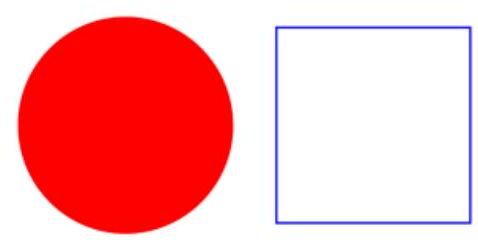
\includegraphics[width=0.2\linewidth]{images/2024_12_29_858f09cde51177c71657g-27}
\end{center}
\end{definition}

\begin{KR}{SVG Grafiken}\\
1. SVG erstellen:
\begin{lstlisting}[language=HTML, style=basesmol]
<svg width="200" height="200">
  <circle cx="100" cy="100" r="50" fill="red"/>
  <rect x="20" y="20" width="50" height="50" fill="blue"/>
</svg>
\end{lstlisting}

2. SVG mit JavaScript manipulieren:
\begin{lstlisting}[language=JavaScript, style=basesmol]
const circle = document.querySelector('circle')
circle.setAttribute('fill', 'green')
circle.setAttribute('r', '60')

// Event Listener fuer SVG-Elemente
circle.addEventListener('click', () => {
  circle.setAttribute('fill', 'yellow')
})
\end{lstlisting}

Vorteile SVG:
\begin{itemize}
  \item Skalierbar ohne Qualitätsverlust
  \item Teil des DOM (manipulierbar)
  \item Gute Browser-Unterstützung
  \item Event-Handler möglich
\end{itemize}
\end{KR}




\begin{examplecode}{SVG mit JavaScript}
\begin{lstlisting}[language=JavaScript, style=basesmol]
// SVG-Element erstellen
const svg = document.createElementNS(
    "http://www.w3.org/2000/svg", 
    "svg"
);
svg.setAttribute("width", "100");
svg.setAttribute("height", "100");

// Kreis hinzufuegen
const circle = document.createElementNS(
    "http://www.w3.org/2000/svg", 
    "circle"
);
circle.setAttribute("cx", "50");
circle.setAttribute("cy", "50");
circle.setAttribute("r", "40");
circle.setAttribute("fill", "red");

svg.appendChild(circle);
\end{lstlisting}
\end{examplecode}

\begin{code}{Wichtige SVG Attribute und Methoden}
\begin{itemize}
  \item \texttt{setAttribute()}: Attribut setzen
  \item \texttt{getAttribute()}: Attribut abfragen
  \item \texttt{removeAttribute()}: Attribut entfernen
  \item \texttt{createElementNS()}: Element erstellen
  \item \texttt{appendChild()}: Element hinzufügen
  \item \texttt{removeChild()}: Element entfernen
  \item \texttt{querySelector()}: Element finden
  \item \texttt{querySelectorAll()}: Alle Elemente finden
  \item \texttt{addEventListener()}: Event-Handler hinzufügen
  \item \texttt{removeEventListener()}: Event-Handler entfernen
  \item \texttt{dispatchEvent()}: Event auslösen
  \item \texttt{createEvent()}: Event erstellen
\end{itemize}
\end{code}

\subsubsection{Canvas}

\begin{definition}{Canvas}
  Das \texttt{<canvas>}-Element bietet eine Zeichenfläche (API) für Pixelgrafiken:
\begin{lstlisting}[language=JavaScript, style=basesmol]
<canvas></canvas>
<script>
  Let cx = document.querySelector("canvas").getContext("2d")
  cx.beginPath()
  cx.moveTo(50, 10)
  cx.lineTo(10, 70)
  cx.lineTo(90, 70)
  cx.fill()
  let img = document.createElement("img")
  img.src = "img/hat.png"
  img.addEventListener("load" , () => {
      for (let x = 10; x < 200; x += 30) {
          cx.drawImage(img, x, 10)
      }
  })
</script>
\end{lstlisting}
\end{definition}


\begin{code}{Canvas Methoden}
  \begin{itemize}
    \item \texttt{scale} - Skalieren
    \item \texttt{translate} - Koordinatensystem verschieben
    \item \texttt{rotate} - Koordinatensystem rotieren
    \item \texttt{save} - Transformationen auf Stack speichern
    \item \texttt{restore} - Letzten Zustand wiederherstellen
  \end{itemize}  
\end{code}


\begin{KR}{Canvas API}
1. Canvas erstellen:
\begin{lstlisting}[language=HTML, style=basesmol]
<canvas id="myCanvas" width="200" height="200"></canvas>
\end{lstlisting}

2. Context holen und zeichnen:
\begin{lstlisting}[language=JavaScript, style=basesmol]
const canvas = document.getElementById('myCanvas')
const ctx = canvas.getContext('2d')

// Rechteck zeichnen
ctx.fillStyle = 'red'
ctx.fillRect(10, 10, 100, 100)

// Pfad zeichnen
ctx.beginPath()
ctx.moveTo(10, 10)
ctx.lineTo(100, 100)
ctx.stroke()

// Text zeichnen
ctx.font = '20px Arial'
ctx.fillText('Hello', 50, 50)

// Bild zeichnen
const img = new Image()
img.onload = () => ctx.drawImage(img, 0, 0)
img.src = 'image.png'
\end{lstlisting}

3. Transformationen:
\begin{lstlisting}[language=JavaScript, style=basesmol]
// Speichern des aktuellen Zustands
ctx.save()

// Transformationen
ctx.translate(100, 100)  // Verschieben
ctx.rotate(Math.PI / 4)  // Rotieren
ctx.scale(2, 2)         // Skalieren

// Zeichnen...

// Wiederherstellen des gespeicherten Zustands
ctx.restore()
\end{lstlisting}

Wichtige Canvas-Methoden:
\begin{itemize}
  \item clearRect(): Bereich löschen
  \item save()/restore(): Kontext speichern/wiederherstellen
  \item translate()/rotate()/scale(): Transformationen
  \item drawImage(): Bilder zeichnen
  \item getImageData()/putImageData(): Pixel-Manipulation
\end{itemize}
\end{KR}







\pagebreak

\subsection{Browser API}

\begin{concept}{Browser-APIs}
    Browser bieten APIs für verschiedene Aufgaben:
    \begin{itemize}
        \item \texttt{localStorage}: Permanente Speicherung
        \item \texttt{sessionStorage}: Daten temporär speichern (aktuelle Session)
        \item \texttt{cookies}: Kleine Datenpakete, auch für Server
        \item \texttt{indexedDB}: NoSQL-Datenbank im Browser
        \item \texttt{history}: Browser-Verlauf
        \item \texttt{location}: URL-Informationen
        \item \texttt{navigator}: Browser-Informationen
        \item \texttt{geolocation}: Standort abfragen
    \end{itemize}
\end{concept}

\begin{definition}{Local Storage}
Mit \texttt{localStorage} können Daten auf dem Client gespeichert werden:
\begin{lstlisting}[language=JavaScript, style=basesmol]
localStorage.setItem("username", "Max")
console.log(localStorage.getItem("username")) // -> Max
localStorage.removeItem("username")
\end{lstlisting}

Local Storage wird verwendet, um Daten der Webseite lokal abzuspeichern. Die Daten bleiben nach dem Schliessen des Browsers erhalten. Die Daten sind in Developer Tools einsehbar und änderbar.

Die Daten werden nach Domains abgespeichert. Es können pro Webseite etwa 5-10MB abgespeichert werden.

Die Werte werden als Strings gespeichert, daher müssen Objekte mit JSON codiert werden:
\begin{lstlisting}[language=JavaScript, style=basesmol]
Let user = {name: "Hans", highscore: 234}
localStorage.setItem(JSON.stringify(user))
\end{lstlisting}
Ausserdem: Synchroner API-Zugriff
\end{definition}


\begin{definition}{Session Storage}
\texttt{sessionStorage} speichert Daten nur für die Dauer der Sitzung:
\begin{lstlisting}[language=JavaScript, style=basesmol]
sessionStorage.setItem("sessionID", "abc123")
\end{lstlisting}
\end{definition}

\begin{KR}{Web Storage} speichert Daten auf der Client-Seite:\\
1. Local Storage (Daten speichern):
\begin{lstlisting}[language=JavaScript, style=basesmol]
// Daten speichern
localStorage.setItem('key', 'value');
localStorage.setItem('user', JSON.stringify({
    name: 'John',
    age: 30
}));
// Daten abrufen
const value = localStorage.getItem('key');
const user = JSON.parse(localStorage.getItem('user'));
// Daten loeschen
localStorage.removeItem('key');
localStorage.clear();  // Alles loeschen
\end{lstlisting}

2. Session Storage (nur für aktuelle Session):
\begin{lstlisting}[language=JavaScript, style=basesmol]
sessionStorage.setItem('key', 'value')
sessionStorage.getItem('key')
sessionStorage.removeItem('key')
\end{lstlisting}
\end{KR}

\begin{definition}{History}
gibt zugriff auf Verlauf des akutellen Fensters/Tab.

\begin{tabular}{|l|l|}
\hline
Methoden & Beschreibung \\
\hline
length (Attribut) & \begin{tabular}{l}
Anzahl Einträgte inkl. aktueller Seite. Keine \\
Methode! \\
\end{tabular} \\
\hline
back & zurück zur letzten Seite \\
\hline
\end{tabular}

\end{definition}

\begin{KR}{History API}
1. Navigation:
\begin{lstlisting}[language=JavaScript, style=basesmol]
// Navigation
history.back()      // Eine Seite zurueck
history.forward()   // Eine Seite vor
history.go(-2)      // 2 Seiten zurueck
\end{lstlisting}

2. History Manipulation:
\begin{lstlisting}[language=JavaScript, style=basesmol]
// Neuen Eintrag hinzufuegen
history.pushState(
  {page: 1},           // State-Objekt
  '',                  // Title (meist ignoriert)
  '/neue-url'          // URL
)

// Aktuellen Eintrag ersetzen
history.replaceState(
  {page: 2},
  '',
  '/andere-url'
)
\end{lstlisting}

3. Auf Änderungen reagieren:
\begin{lstlisting}[language=JavaScript, style=basesmol]
window.addEventListener('popstate', (event) => {
  console.log(event.state)    // State-Objekt
  console.log(location.href)  // Aktuelle URL
})
\end{lstlisting}
\end{KR}

\begin{definition}{Cookies}
    Cookies sind kleine Datenpakete, die im Browser gespeichert werden:
    \begin{itemize}
        \item \texttt{document.cookie}: Cookies lesen/schreiben
        \item \texttt{expires}: Ablaufdatum
        \item \texttt{path}: Pfad, für den das Cookie gültig ist
        \item \texttt{domain}: Domain, für die das Cookie gültig ist
        \item \texttt{secure}: Nur über HTTPS
    \end{itemize}
\end{definition}

\begin{code}{GeoLocation}\\
Mit der GeoLocation-API kann der Standort abgefragt werden.

\begin{lstlisting}[language=JavaScript, style=basesmol]
var options = { enableHighAccuracy: true, timeout: 5000, maximumAge: 0 }
function success(pos) {
    var crd = pos.coords
    console.log(`Latitude : ${crd.latitude}`)
    console.log(`Longitude: ${crd.longitude}`)
    console.log(`More or less ${crd.accuracy} meters.`)
}
function error(err) { ... }
navigator.geolocation.getCurrentPosition(success, error, options)
\end{lstlisting}
\end{code}


\begin{KR}{Geolocation API}
1. Einmalige Position abfragen:
\begin{lstlisting}[language=JavaScript, style=basesmol]
navigator.geolocation.getCurrentPosition(
  (position) => {
    console.log(position.coords.latitude)
    console.log(position.coords.longitude)
    console.log(position.coords.accuracy)
  },
  (error) => {
    console.error(error.message)
  },
  {
    enableHighAccuracy: true,
    timeout: 5000,
    maximumAge: 0
  }
)
\end{lstlisting}

2. Position kontinuierlich überwachen:
\begin{lstlisting}[language=JavaScript, style=basesmol]
const watchId = navigator.geolocation.watchPosition(
  positionCallback,
  errorCallback,
  options
)

// Ueberwachung beenden
navigator.geolocation.clearWatch(watchId)
\end{lstlisting}
\end{KR}



\begin{KR}{Web Workers}
1. Worker erstellen:
\begin{lstlisting}[language=JavaScript, style=basesmol]
// main.js
const worker = new Worker('worker.js')

worker.postMessage({data: someData})

worker.onmessage = (e) => {
  console.log('Nachricht vom Worker:', e.data)
}

// worker.js
self.onmessage = (e) => {
  // Daten verarbeiten
  const result = doSomeHeavyComputation(e.data)
  self.postMessage(result)
}
\end{lstlisting}

2. Worker beenden:
\begin{lstlisting}[language=JavaScript, style=basesmol]
worker.terminate()  // Im Hauptthread
self.close()       // Im Worker
\end{lstlisting}

Wichtig:
\begin{itemize}
  \item Worker laufen in separatem Thread
  \item Kein Zugriff auf DOM
  \item Kommunikation nur über Nachrichten
  \item Gut für rechenintensive Aufgaben
\end{itemize}
\end{KR}

\pagebreak

\subsection{Client-Server-Interaktion (Formulare)}

\subsubsection{Formular Events}

\begin{definition}{Formulare}
Formulare ermöglichen Benutzereingaben. Sie gilt als Grundlade für Interaktion mit dem Web.\\
Input types:

\begin{itemize}
\item submit, number, text, password, email, url , range , date , search , color
\end{itemize}
\end{definition}



\begin{definition}{HTML-Formulare}\\
    Formulare ermöglichen Benutzereingaben und Datenübertragung:
    \begin{itemize}
        \item \texttt{<form>} Element mit \texttt{action} und \texttt{method}
        \item \texttt{method="GET"}: Daten in URL (sichtbar)
        \item \texttt{method="POST"}: Daten im Request-Body (unsichtbar)
        \item Verschiedene Input-Typen: text, password, checkbox, radio, etc.
    \end{itemize}
\end{definition}

\begin{KR}{Formular Handling}
1. Formular erstellen:
\begin{lstlisting}[language=HTML, style=basesmol]
<form action="/api/submit" method="post">
  <input type="text" name="username">
  <input type="password" name="password">
  <button type="submit">Login</button>
</form>
\end{lstlisting}

2. Formular Events abfangen:
\begin{lstlisting}[language=JavaScript, style=basesmol]
form.addEventListener("submit", (e) => {
  e.preventDefault() 
  // Eigene Verarbeitung
})
\end{lstlisting}

3. Formulardaten verarbeiten:
\begin{lstlisting}[language=JavaScript, style=basesmol]
const formData = new FormData(form)
fetch("/api/submit", {
  method: "POST",
  body: formData
})
\end{lstlisting}
\end{KR}

\subsubsection{Event Handling für Formulare}

\begin{formula}{Formular Events}
    Wichtige Events bei Formularen:
    \begin{itemize}
        \item \texttt{submit}: Formular wird abgeschickt
        \item \texttt{reset}: Formular wird zurückgesetzt
        \item \texttt{change}: Wert eines Elements wurde geändert
        \item \texttt{input}: Wert wird gerade geändert
        \item \texttt{focus}: Element erhält Fokus
        \item \texttt{blur}: Element verliert Fokus
    \end{itemize}
\end{formula}

\begin{definition}{Default-Verhalten}
Das Default-Verhalten von Formularen kann mit \texttt{preventDefault()} unterbunden werden.
\begin{lstlisting}[language=JavaScript, style=basesmol]
let form = document.querySelector("form");
form.addEventListener("submit", event => {
    event.preventDefault();
    console.log("Formular abgesendet!");
});
\end{lstlisting}
\end{definition}

\begin{KR}{Formular Handling}
\begin{lstlisting}[language=JavaScript, style=basesmol]
// HTML Formular erstellen
<form action="/submit" method="POST">
    <label for="username">Username:</label>
    <input type="text" id="username" name="username">
    
    <label for="password">Password:</label>
    <input type="password" id="password" name="password">
    
    <button type="submit">Login</button>
</form>

// JavaScript Handler
form.addEventListener('submit', (event) => {
    event.preventDefault(); // Verhindert Standard-Submit
    
    const formData = new FormData(form);
    // Zugriff auf Formular-Daten
    const username = formData.get('username');
    const password = formData.get('password');
    
    // Mit Fetch API senden
    fetch('/submit', {
        method: 'POST',
        body: formData
    });
});
\end{lstlisting}
\end{KR}






\subsubsection{GET/POST Methode}

Formulare können auch POST/GET Aktionen ausführen:\\
Action beschreibt das Skript, welches die Daten annimmt. Method ist die Methode die ausgeführt wird.

\begin{lstlisting}[language=JavaScript, style=basesmol]
<form action="/login" method="post">
2 ...
3 </form>
\end{lstlisting}

\begin{center}
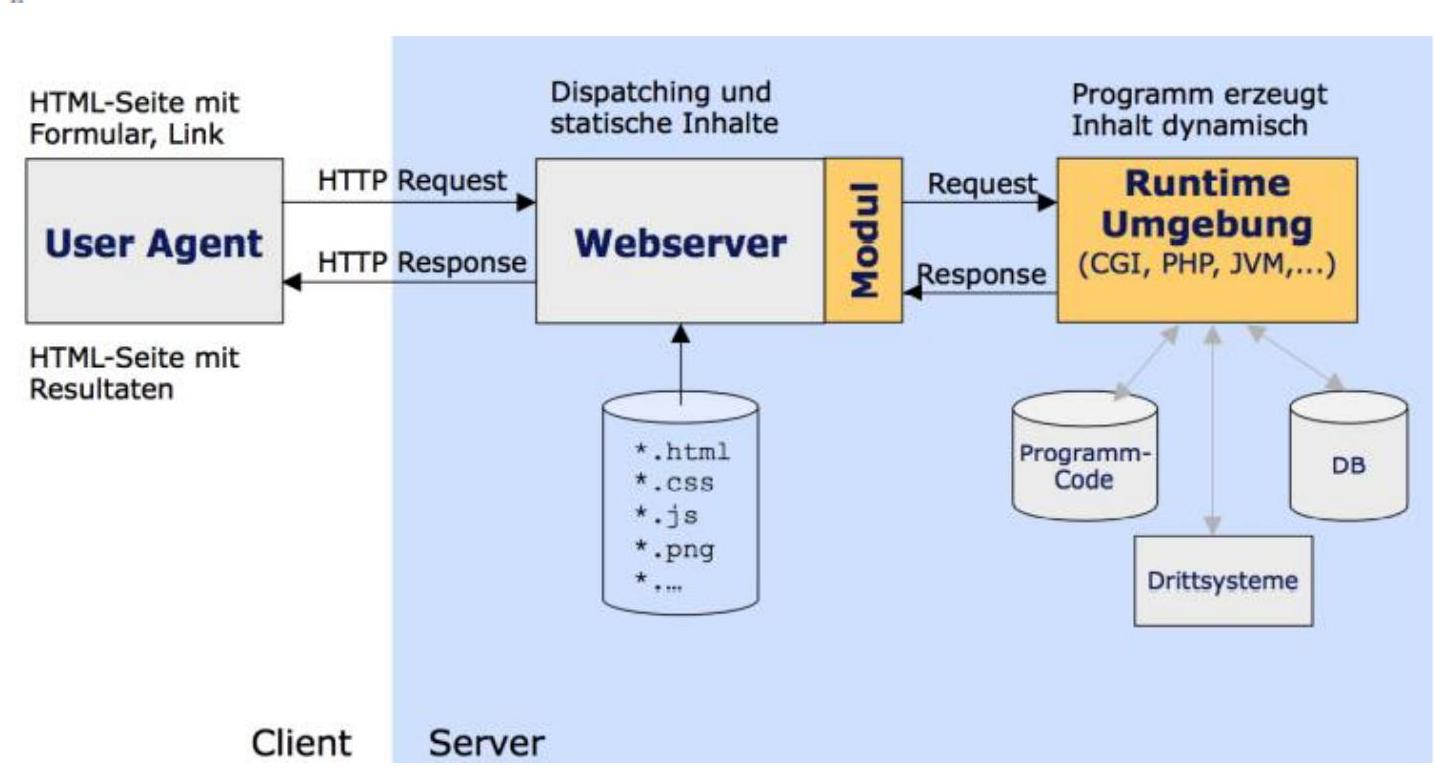
\includegraphics[width=\linewidth]{images/2024_12_29_858f09cde51177c71657g-29(1)}
\end{center}




\begin{example2}{Formulare}
\begin{lstlisting}[language=JavaScript, style=basesmol]
<form>
  <fieldset>
      <legend>General information</legend>
      <label>Text field <input type="text" value="hi"></label>
      <label>Password <input type="password" value="hi"></label>
      <label class="area">Textarea <textarea>hi</textarea></label>
  </fieldset>
  <fieldset>
      <legend>Additional information</legend>
      <label>Checkbox <input type="checkbox"></label>
      <label>Radio button <input type="radio" name="demo" checked></label>
      <label>Another one <input type="radio" name="demo"></label>
  </fieldset>
  <form>
  <label>Button <button>Click me</button></label>
  <label>Select menu
  <select name="cars">
  <option value="volvo">Volvo</option>
  <option value="saab">Saab</option>
  <option value="fiat">Fiat</option>
  <option value="audi">Audi</option>
  </select>
  </label>
  <input type="submit" value="Send">
</form>
|'
\end{lstlisting}



\begin{center}
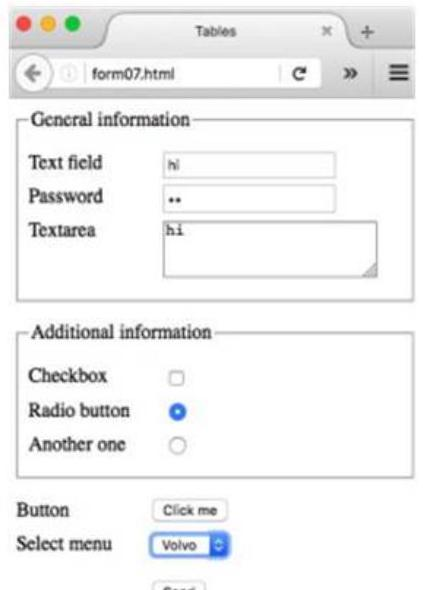
\includegraphics[width=0.5\linewidth]{images/2024_12_29_858f09cde51177c71657g-29}
\end{center}
\end{example2}

\pagebreak

\subsection{Cookies und Sessions}





\begin{definition}{HTTP-Cookies}

\begin{itemize}
\item HTTP als zustandsloses Protokoll konzipiert
\item Cookies: Speichern von Informationen auf dem Client
\item Response: Set-Cookie -Header, Request: Cookie -Header
\item Zugriff mit JavaScript möglich (ausser HttpOnly ist gesetzt)\\
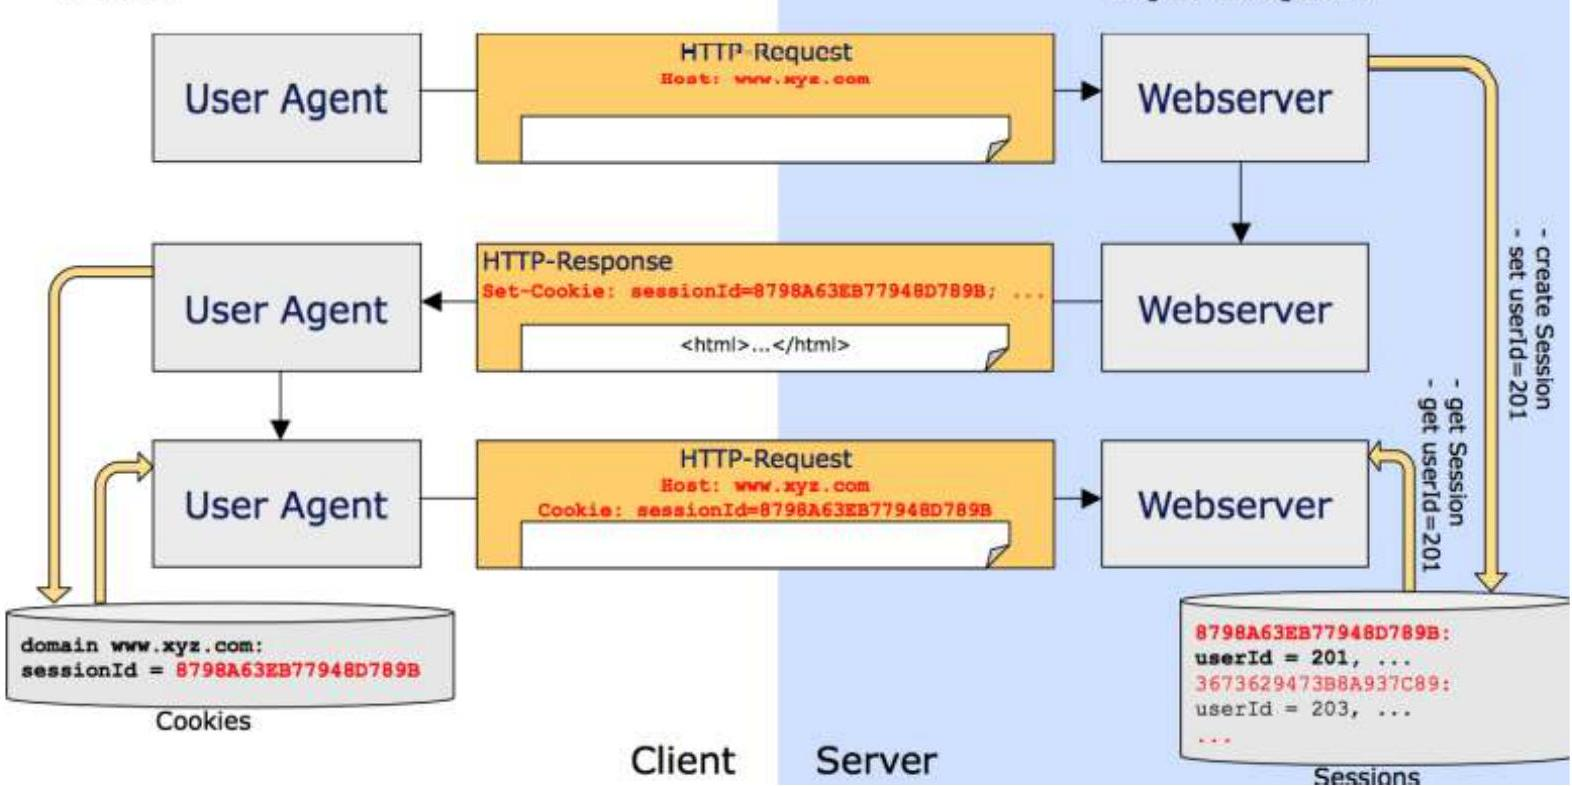
\includegraphics[width=\linewidth]{images/2024_12_29_858f09cde51177c71657g-31(1)}
\end{itemize}
\end{definition}

\begin{definition}{Cookies}
Cookies speichern clientseitig Daten:
\begin{lstlisting}[language=JavaScript, style=basesmol]
document.cookie = "username=Max; expires=Fri, 31 Dec 2025 23:59:59 GMT";
console.log(document.cookie);
\end{lstlisting}
HTTP-Cookies sind kleine Datenpakete:
\begin{itemize}
    \item Werden vom Server gesetzt
    \item Im Browser gespeichert
    \item Bei jedem Request mitgesendet
    \item Haben Name, Wert, Ablaufdatum und Domain
\end{itemize}
\end{definition}


\begin{KR}{Cookie Handling}
1. Cookie setzen:
\begin{lstlisting}[language=JavaScript, style=basesmol]
document.cookie = "username=Max; expires=Fri, 31 Dec 2024 23:59:59 GMT; path=/"
\end{lstlisting}

2. Cookies lesen:
\begin{lstlisting}[language=JavaScript, style=basesmol]
function getCookie(name) {
  const value = `; ${document.cookie}`
  const parts = value.split(`; ${name}=`)
  if (parts.length === 2) return parts.pop().split(';').shift()
}
\end{lstlisting}

3. Cookie löschen:
\begin{lstlisting}[language=JavaScript, style=basesmol]
document.cookie = "username=; expires=Thu, 01 Jan 1970 00:00:00 GMT; path=/"
\end{lstlisting}

Wichtige Cookie-Attribute:
\begin{itemize}
  \item expires/max-age: Gültigkeitsdauer
  \item path: Gültigkeitspfad
  \item secure: Nur über HTTPS
  \item httpOnly: Kein JavaScript-Zugriff
  \item samesite: Cross-Site-Cookie-Verhalten
\end{itemize}
\end{KR}

\begin{KR}{Cookie Handling}
\begin{lstlisting}[language=JavaScript, style=basesmol]
// Cookie setzen
document.cookie = "username=John Doe; expires=Thu, 18 Dec 2024 12:00:00 UTC; path=/";

// Cookie lesen
const cookies = document.cookie.split(';').reduce((acc, cookie) => {
    const [name, value] = cookie.trim().split('=');
    acc[name] = value;
    return acc;
}, {});

// Cookie loeschen
document.cookie = "username=; expires=Thu, 01 Jan 1970 00:00:00 UTC; path=/;";
\end{lstlisting}
\end{KR}

\begin{concept}{Sessions}
    Server-seitige Speicherung von Benutzerdaten:
    \begin{itemize}
        \item Session-ID wird in Cookie gespeichert
        \item Daten bleiben auf dem Server
        \item Sicherer als Cookies für sensible Daten
        \item Temporär (bis Browser geschlossen wird)
    \end{itemize}
\end{concept}

\begin{definition}{Sessions}
\begin{itemize}
\item Cookies auf dem Client leicht manipulierbar
\item Session: Client-spezifische Daten auf dem Server speichern
\item Identifikation des Clients über Session-ID (Cookie o.a.)
\item Gefahr: Session-ID gerät in falsche Hände (Session-Hijacking)
\end{itemize}
\end{definition}



\begin{definition}{Sessions}
Sessions speichern serverseitig Daten und nutzen eine Session-ID für die Zuordnung:
\begin{lstlisting}[language=JavaScript, style=basesmol]
// Beispiel: Session-Handling mit Express.js
req.session.user = "Max";
console.log(req.session.user);
\end{lstlisting}
\end{definition}

\pagebreak

\subsection{AJAX und Fetch API}

\begin{concept}{AJAX}
    Asynchronous JavaScript And XML:
    \begin{itemize}
        \item Asynchrone Kommunikation mit dem Server
        \item Kein vollständiges Neuladen der Seite nötig
        \item Moderne Alternative: Fetch API
        \item Datenformate: JSON, XML, Plain Text
    \end{itemize}
\end{concept}

\begin{definition}{Fetch API}
Mit der Fetch-API können HTTP-Requests ausgeführt werden:
\begin{lstlisting}[language=JavaScript, style=basesmol]
fetch("/data.json")
  .then(response => response.json())
  .then(data => console.log(data))
  .catch(error => console.error("Fehler:", error))
\end{lstlisting}
\begin{itemize}
\item HTTP-Requests von JavaScripts
\item Geben Promise zurück
\item Nach Server-Antwort erfüllt mit Response-Objekt
\end{itemize}
\end{definition}


\begin{lstlisting}[language=JavaScript, style=basesmol]
fetch("example/data.txt")
.then(response => {
          console.log(response.status) // -> 200
  console.log(response.headers.get("Content-Type")) // -> text/plain
})
.then(resp => resp.text())
.then(text => console.log(text))
// -> This is the content of data.txt
\end{lstlisting}

\begin{definition}{Response Objekt}

\begin{itemize}
\item headers : Zugriff auf HTTP-Header-Daten Methoden get, keys, forEach , ...
\item status: Status-Code
\item json() : liefert Promise mit Resultat der JSON-Verarbeitung
\item text() : liefert Promise mit Inhalt der Server-Antwort
\end{itemize}
\end{definition}


\begin{concept}{XMLHttpRequest und Fetch}
    Moderne Ansätze für HTTP-Requests:
    \begin{itemize}
        \item XMLHttpRequest: Älterer Ansatz, komplexer
        \item Fetch API: Moderner Ansatz, Promise-basiert
        \item Unterstützung für verschiedene Datenformate
        \item CORS (Cross-Origin Resource Sharing)
    \end{itemize}
\end{concept}

\begin{KR}{Fetch API Grundlagen}
\begin{lstlisting}[language=JavaScript, style=basesmol]
// GET Request
fetch('https://api.example.com/data')
    .then(response => {
        if (!response.ok) {
            throw new Error('Network response was not ok');
        }
        return response.json();
    })
    .then(data => console.log(data))
    .catch(error => console.error('Error:', error));

// POST Request
fetch('https://api.example.com/data', {
    method: 'POST',
    headers: {
        'Content-Type': 'application/json',
    },
    body: JSON.stringify({
        key: 'value'
    })
})
    .then(response => response.json())
    .then(data => console.log(data));

// Mit async/await
async function fetchData() {
    try {
        const response = await fetch('https://api.example.com/data');
        if (!response.ok) {
            throw new Error('Network response was not ok');
        }
        const data = await response.json();
        return data;
    } catch (error) {
        console.error('Error:', error);
    }
}
\end{lstlisting}
\end{KR}



\begin{KR}{HTTP Requests mit Fetch}\\
1. GET Request:
\begin{lstlisting}[language=JavaScript, style=basesmol]
fetch("/api/data")
  .then(response => response.json())
  .then(data => console.log(data))
  .catch(error => console.error(error))
\end{lstlisting}

2. POST Request:
\begin{lstlisting}[language=JavaScript, style=basesmol]
fetch("/api/create", {
  method: "POST",
  headers: {
    "Content-Type": "application/json"
  },
  body: JSON.stringify(data)
})
\end{lstlisting}

3. Mit async/await:
\begin{lstlisting}[language=JavaScript, style=basesmol]
async function getData() {
  try {
    const response = await fetch("/api/data")
    const data = await response.json()
    return data
  } catch (error) {
    console.error(error)
  }
}
\end{lstlisting}
\end{KR}



\begin{concept}{CORS (Cross-Origin Resource Sharing)}
    Sicherheitsmechanismus für domainübergreifende Requests:
    \begin{itemize}
        \item Verhindert unauthorized Zugriffe
        \item Server muss CORS-Header setzen
        \item Preflight Requests für bestimmte Anfragen
        \item Wichtige Header:
            \begin{itemize}
                \item Access-Control-Allow-Origin
                \item Access-Control-Allow-Methods
                \item Access-Control-Allow-Headers
            \end{itemize}
    \end{itemize}
\end{concept}

\begin{KR}{Sessions und Authentication}
\begin{lstlisting}[language=JavaScript, style=basesmol]
// Login Request
async function login(username, password) {
    const response = await fetch('/api/login', {
        method: 'POST',
        headers: {
            'Content-Type': 'application/json',
        },
        credentials: 'include',  // Fuer Cookies
        body: JSON.stringify({
            username,
            password
        })
    });
    
    if (response.ok) {
        const user = await response.json();
        // Session Token in localStorage speichern
        localStorage.setItem('token', user.token);
    }
}

// Authenticated Request
async function getProtectedData() {
    const token = localStorage.getItem('token');
    const response = await fetch('/api/protected', {
        headers: {
            'Authorization': `Bearer ${token}`
        }
    });
    return response.json();
}
\end{lstlisting}
\end{KR}

\begin{concept}{WebSocket}
    Bidirektionale Echtzeit-Kommunikation:
    \begin{itemize}
        \item Permanente Verbindung
        \item Geringer Overhead
        \item Ideal für Chat, Live-Updates
        \item Events: open, message, close, error
    \end{itemize}

\begin{lstlisting}[language=JavaScript, style=basesmol]
const ws = new WebSocket('ws://localhost:8080');

ws.addEventListener('open', () => {
    console.log('Connected to WebSocket');
    ws.send('Hello Server!');
});

ws.addEventListener('message', event => {
    console.log('Received:', event.data);
});

ws.addEventListener('close', () => {
    console.log('Disconnected from WebSocket');
});
\end{lstlisting}
\end{concept}

\columnbreak

\subsection{REST APIs}

\begin{definition}{REST Prinzipien}
    Representational State Transfer:
    \begin{itemize}
        \item Zustandslos (Stateless)
        \item Ressourcen-orientiert
        \item Einheitliche Schnittstelle
        \item Standard HTTP-Methoden
    \end{itemize}
\end{definition}

\begin{KR}{REST API Implementierung} mit Fetch API:
\begin{lstlisting}[language=JavaScript, style=basesmol]
// GET - Daten abrufen
fetch('/api/users')
    .then(response => response.json())
    .then(users => console.log(users));

// POST - Neue Ressource erstellen
fetch('/api/users', {
    method: 'POST',
    headers: {
        'Content-Type': 'application/json',
    },
    body: JSON.stringify({
        name: 'John',
        email: 'john@example.com'
    })
});

// PUT - Ressource aktualisieren
fetch('/api/users/123', {
    method: 'PUT',
    headers: {
        'Content-Type': 'application/json',
    },
    body: JSON.stringify({
        name: 'John Updated'
    })
});

// DELETE - Ressource loeschen
fetch('/api/users/123', {
    method: 'DELETE'
});
\end{lstlisting}
\end{KR}

\begin{KR}{REST API Implementierung mit Express}
\begin{lstlisting}[language=JavaScript, style=basesmol]
const express = require('express');
const app = express();
app.use(express.json());

// GET - Alle Benutzer abrufen
app.get('/api/users', (req, res) => {
    res.json(users);
});

// GET - Einzelnen Benutzer abrufen
app.get('/api/users/:id', (req, res) => {
    const user = users.find(u => u.id === parseInt(req.params.id));
    if (!user) return res.status(404).send('User not found');
    res.json(user);
});

// POST - Neuen Benutzer erstellen
app.post('/api/users', (req, res) => {
    const user = {
        id: users.length + 1,
        name: req.body.name
    };
    users.push(user);
    res.status(201).json(user);
});

// PUT - Benutzer aktualisieren
app.put('/api/users/:id', (req, res) => {
    const user = users.find(u => u.id === parseInt(req.params.id));
    if (!user) return res.status(404).send('User not found');
    
    user.name = req.body.name;
    res.json(user);
});

// DELETE - Benutzer loeschen
app.delete('/api/users/:id', (req, res) => {
    const user = users.find(u => u.id === parseInt(req.params.id));
    if (!user) return res.status(404).send('User not found');
    
    const index = users.indexOf(user);
    users.splice(index, 1);
    res.json(user);
});
\end{lstlisting}
\end{KR}



